% Created 2019-02-03 Sun 23:33
% Intended LaTeX compiler: pdflatex
\documentclass[a4paper, twoside, 12pt]{article}
\usepackage[utf8]{inputenc}
\usepackage[T1]{fontenc}
\usepackage{graphicx}
\usepackage{grffile}
\usepackage{longtable}
\usepackage{wrapfig}
\usepackage{rotating}
\usepackage[normalem]{ulem}
\usepackage{amsmath}
\usepackage{textcomp}
\usepackage{amssymb}
\usepackage{capt-of}
\usepackage{hyperref}
\usepackage[left=2.5cm, right=2.5cm, top=2.5cm, bottom=2.5cm, bindingoffset=1.5cm, head=15pt]{geometry}
\usepackage{setspace}
\usepackage{caption}
\onehalfspacing
\usepackage[official]{eurosym}
\usepackage{amsmath}
\usepackage{amssymb}
\usepackage{notation}
\usepackage{fancyhdr}
\pagestyle{fancy}
\fancyhead{}
\fancyfoot{}
\fancyhead[LE,RO]{\textsl{\leftmark}}
\fancyhead[RE,LO]{Tobias Richter}
\fancyfoot[C]{\thepage}
\renewcommand{\headrulewidth}{0.4pt}
\renewcommand{\footrulewidth}{0pt}
\usepackage{apacite}
\let\cite\shortcite
\let\textcite\shortciteA
\usepackage[numbib,notlof,notlot,nottoc]{tocbibind}
\newcommand{\studentID}{558305}
\newcommand{\thesistype}{Master Thesis}
\newcommand{\supervisor}{Univ.-Prof. Dr. Wolfgang Ketter}
\newcommand{\cosupervisor}{Karsten Schroer, Philipp Arthur Kienscherf}
\pagenumbering{Roman}
\author{Tobias Richter}
\date{\today}
\title{Reinforcement Learning Portfolio Optimization of Electric Vehicle Virtual Power Plants}
\hypersetup{
 pdfauthor={Tobias Richter},
 pdftitle={Reinforcement Learning Portfolio Optimization of Electric Vehicle Virtual Power Plants},
 pdfkeywords={},
 pdfsubject={},
 pdfcreator={Emacs 26.1 (Org mode 9.2)},
 pdflang={English}}
\begin{document}

\makeatletter
\begin{titlepage}
    \begin{center}
        \vspace*{1cm}

        \Large
        \textbf{\@title{}}

        \vspace{1.5cm}

        \thesistype{}

        \vspace{1cm}

        \begin{figure}[htbp]
             \centering
             
\includegraphics[width=.5\linewidth]{./fig/UoC_Logo.png}
        \end{figure}

        \vspace{1cm}

        \large
        \textbf{Author}: \@author{} (Student ID: \studentID{})\\
        \large
        \textbf{Supervisor}: \supervisor{}\\
        \large
        \textbf{Co-Supervisor}: \cosupervisor{}

        \vspace{1cm}
        \large
        Department of Information Systems for Sustainable Society\\
        Faculty of Management, Economics and Social Sciences\\
        University of Cologne\\

        \vspace{1cm}
        \@date{}

    \end{center}
\end{titlepage}
\makeatother
\clearpage

\thispagestyle{empty}
\section*{Eidesstattliche Versicherung}
\label{sec:SOOA}

\vspace{2.5cm}

% Statement of original authorship - Needs to be in German
% see also here: https://www.wiso.uni-koeln.de/sites/fakultaet/dokumente/PA/formulare/eidesstattliche_erklaerung.pdf

Hiermit versichere ich an Eides statt, dass ich die vorliegende Arbeit selbstständig und ohne die Benutzung anderer als der angegebenen Hilfsmittel angefertigt habe. Alle Stellen, die wörtlich oder sinngemäß aus veröffentlichten und nicht veröffentlichten Schriften entnommen wurden, sind als solche kenntlich gemacht. Die Arbeit ist in gleicher oder ähnlicher Form oder auszugsweise im Rahmen einer anderen Prüfung noch nicht vorgelegt worden. Ich versichere, dass die eingereichte elektronische Fassung der eingereichten Druckfassung vollständig entspricht.

\vspace{1cm}

\noindent
Die Strafbarkeit einer falschen eidesstattlichen Versicherung ist mir bekannt, namentlich die Strafandrohung gemäß § 156 StGB bis zu drei Jahren Freiheitsstrafe oder Geldstrafe bei vorsätzlicher Begehung der Tat bzw. gemäß § 161 Abs. 1 StGB bis zu einem Jahr Freiheitsstrafe oder Geldstrafe bei fahrlässiger Begehung.

\vspace{3cm}
\noindent
\textbf{\@author{}}

\vspace{0.5cm}
\noindent
Köln, den xx.xx.20xx
\clearpage

\setcounter{page}{1}
\tableofcontents
\clearpage
\listoffigures
\clearpage
\listoftables
\clearpage
\pagenumbering{arabic}

\section{Introduction (10\%)}
\label{sec:org817e467}
\subsection{Research Motivation}
\label{sec:orgc23d056}
\begin{itemize}
\item \cite{lopes11_integ_elect_vehic_elect_power_system}
\end{itemize}
\subsection{Research Question}
\label{sec:org001a4f7}
\subsection{Relevance}
\label{sec:org21be2fe}

\clearpage
\section{Related Literature (10\%)}
\label{sec:org5b19ead}
\subsection{Smart Charging and Balancing the Electric Grid with EV Fleets}
\label{sec:orgb0dce67}
The increasing penetration of EVs has a substantial effect on electricity
consumption patterns. During charging periods, power flows and grid losses
increase considerably and challenge the grid. Operators have to reinforce the
grid to ensure that transformers and substations do not get overloaded
\cite{sioshansi12_impac_elect_tarif_plug_in,lopes11_integ_elect_vehic_elect_power_system}.
Loading multiple EVs in the same neighborhood, or worse, whole EV fleets at
once, stress the grid. In these cases, even brown- or blackouts are possible
\cite{kim12_carbit}. Despite these challenges, it is possible to postpone the
physical reinforcement by adopting smart charging strategies. In smart charging,
EVs get charged when the grid is less congested to achieve more grid stability.
Smart charging reduces peaks in electricity demand, called \emph{Peak Cutting} and
complement the grid in times of low demand, called \emph{Valley Filling}. Smart
charging has been researched thoroughly in the IS literature, in the following
we will outline some of the most important contributions.

\textcite{valogianni14_effec_manag_elect_vehic_storag} find that using intelligent
agents to schedule EV charging substantially reshapes the energy demand and
reduces peak demand without violating individual household preferences.
Moreover, they show that the proposed smart charging behavior reduced average
energy prices and thus economically benefit households. In another study
\textcite{kara15_estim_benef_elect_vehic_smart} investigate the effect of smart
charging on public charging stations in California. Controlling for arrival and
departure times, the authors present beneficial results for the distribution
system operator (DSO) and the owners of EVs. A price reduction in energy bills
and a peak load reduction could be determined. An extension of the smart
charging concept is Vehicle-to-Grid (V2G). When equipped with V2G devices, EVs
can discharge their batteries back into the grid. Several authors researched
this technology in respect to grid stabilization effects and arbitrage
possibilities. \textcite{schill11_elect_vehic_imper_elect_market} find that EVs
can be beneficial for average consumer electricity prices. Excess EV battery
capacity can be used to charge in off-peak hours and discharge in peak hours
when the prices are higher. These arbitrage possibilities reverse welfare
effects of generators and increase general overall welfare and consumer surplus.
\textcite{tomic07_using_fleet_elect_drive_vehic_grid_suppor} show that the
arbitrage opportunities are especially prominent when a high variability in
electricity prices on the target electricity market exists. The authors state
that short intervals between the contract of sale and the physical delivery of
electricity increase arbitrage benefits. Consequently, ancillary service
markets, like frequency control and operating reserve markets, are attractive
for smart charging.

\textcite{peterson10_econom_using_plug_in_hybrid} investigate energy arbitrage
profitability with V2G in the light of battery depreciation costs in the US.
Their results indicate that large-scale use of EV batteries for grid storage
does not yield enough profits to incentivize EV owners to participate in V2G
activities. Considering battery depreciation cost, they arrive at an annual
profit of only 6\$ - 72\$ per EV.
\textcite{brandt17_evaluat_busin_model_vehic_grid_integ} evaluated a business
model for parking garage operators operating on the German frequency regulation
market. When taking infrastructure costs and battery depreciation costs into
account, they concluded that the proposed vehicle-grid integration is not
profitable. Even with generous assumptions about EV adoption rates in Germany
and altered auction mechanisms they arrived at negative profits.
\textcite{kahlen17_fleet} used EV fleets to offer balancing services to the grid.
Evaluating the impact of V2G in their model the authors conclude that V2G would
only be profitable if reserve power prices would be twice as high. Considering
the results from the studies mentioned above this research does not include V2G
is the model, only marginal profits are expected.

In order to maximize profits, it is essential for market participants to develop
good bidding strategies. Successful bidding strategies to jointly participate in
multiple markets have been developed, e.g., by
\textcite{mashhour11_biddin_strat_virtual_power_plant_2}. The authors use
stationary battery storage to participate in the spinning reserve market and the
day-ahead market at the same time. They developed a non-equilibrium model, which
solves the presented mixed-integer program with Genetic Programming (GP).
Contrarily, we use a model-free RL agent that learns an optimal policy (i.e., a
trading strategy) from actions it takes in the environment (i.e., bidding on
electricity markets). Using a model-free approach is especially beneficial for
us, since additional unknown variables and constraints (i.e., customer mobility
demand), make it complicated to formulate a mathematical model.

\textcite{he16_optim_biddin_strat_batter_storag} have done similar research to
\textcite{mashhour11_biddin_strat_virtual_power_plant_2}. The authors additionally
incorporate battery life cycle in their profit maximization model, which proves
to be a decisive factor. In contrast to the authors, we jointly participated in
the secondary operating reserve and spot market with the \emph{non-stationary}
storage of EV batteries. Because shared EVs have to satisfy mobility demands,
they have to be charged in any case, which allows us to safely exclude battery
deprecation from our model. Further, we chose the intraday market over the
day-ahead market, as it has the lowest reaction time of the spot markets, and
thus potentially offers higher profits
\cite{tomic07_using_fleet_elect_drive_vehic_grid_suppor}.

Previous studies often assume that car owners or households can directly trade
on electricity markets. In reality, this is not possible due to the minimum
capacity requirements of the markets, that single EVs do not meet. For example,
the German Control Reserve Market (GCRM) has a minimum trading capacity of 1MW
to 5MW, depending on the specific market. In order to reach the minimum
capacity, over 200 EVs would need to be connected to the grid via a standard
4.6kW charging station at the same time. \textcite{ketter13_power_tac} introduced
the notion of electricity brokers, aggregators that act on behalf of a group of
individuals or households to participate in electricity markets.
\textcite{brandt17_evaluat_busin_model_vehic_grid_integ} and
\textcite{kahlen14_balan_with_elect_vehic} successfully showed in their studies
that electricity brokers could overcome the capacity issues by aggregating EV
batteries. In addition to electricity brokers, we apply the concept of Virtual
Power Plants (VPPs). VPPs are flexible portfolios of distributed energy
resources, which are presented with a single load profile to the system
operator, making them eligible for market participation and ancillary service
provisioning \cite{pudjianto07_virtual_power_plant_system_integ}. Hence, VPPs
allow providing regulation capacity to the market without knowing which exact
sources provide the promised capacity until the delivery time
\cite{kahlen17_fleet}. This concept is specially useful when dealing with EV
fleets: VPPs enable carsharing providers to issue bids and asks based on an
estimate of available fleet capacity, without knowing beforehand which exact EVs
will provide the capacity at the time of delivery. Based on the battery charge
and the availability EVs, an intelligent agent will decide in real-time which
vehicles provide the capacity.

Carsharing providers manage large EV fleets, which makes it possible for them to
use the presented concepts as a viable business extension. Free float carsharing
is a popular concept where which allows cars to be picked up and parked
everywhere, and the customers are billed is by the minute. Free float carsharing
offers more flexibility to its users, saves resources and reduces carbon
emissions \cite{firnkorn15_free_float_elect_carsh_fleet_smart_cities}. Most
previous studies concerned with using EVs for electricity trading, assumed that
trips are fixed and known in advance, e.g., in
\textcite{tomic07_using_fleet_elect_drive_vehic_grid_suppor}. The free float
concept adds uncertainty and nondeterministic behavior, which make predictions
about future rentals a complex issue.

\textcite{kahlen17_fleet} showed that it is possible to use free float carsharing
fleets as VPPs to profitably offer balancing services to the grid. The authors
compared cases from three different cities across Europe and the US. They used
an event-based simulation, bootstrapped with real-world carsharing and secondary
operating reserve market data from the respective cities, to arrive at their
results. A central dilemma within this research is to decide whether an EV
should be committed to a VPP or to be free for rent, in the core a
classification problem. Since rental profits are considerably higher than
profits from electricity trading, it is crucial not to allocate an EV to a VPP
when it could have been rented out otherwise. To deal with the asymmetric
payoff, \citeauthor{kahlen17_fleet} use stratified sampling in their classifier.
This method gives rental misclassifications higher weights, which reduces the
likelihood of EVs to participate in VPP activities. The authors use a Random
Forest regression model to predict the available balancing capacity, which they
use to place bids and asks on the market. An agent predicts available capacity
on an aggregated fleet level, in order to leverage risk-pooling effects. Only at
the delivery time the agent decides which EVs will provide the regulation
capacity based on the likelihood that the vehicle is rented out and on the
expected benefits of the EV. In a similar study, the authors showed that
carsharing companies could participate in day-ahead markets for arbitrage
purposes \cite{kahlen18_elect_vehic_virtual_power_plant_dilem}. In this
paper, the authors use a time-series model to predict available trading
capacity, due to less time between commitment and delivery. Another central
problem for the carsharing provider is that committed trades which can not be
fulfilled result in substantial penalties from the system operator or
electricity exchange. In other words, it should be avoided at all costs, that
the fleet commits to buy any amount of electricity, for which it does not have
enough available EVs to charge it at the delivery time. To address this issue,
the authors develop a mean asymmetric weighted (MAW) objective function. They
use it for their time-series based prediction model, to penalize committing an
EV to VPP when it would have been rented out otherwise. Because of the two
issues mentioned above, \textcite{kahlen18_elect_vehic_virtual_power_plant_dilem}
can only make very conservative estimations and commitments of overall available
trading capacity, which results in a high amount of foregone profits. This
effect is especially prominent when participating in the secondary operating
reserve market since commitments have to be made one week in advance when
mobility demands are still uncertain. \textcite{kahlen17_fleet} state that in 42\%
to 80\% of the cases EVs are \emph{not} committed to a VPP when it would have been
profitable to do so.

This research is proposing a solution, in which the EV fleet participates in the
balancing market and intraday market simultaneously. With this approach, we
align the potentially higher profits on the balancing markets, with more
accurate capacity predictions for intraday markets
\cite{tomic07_using_fleet_elect_drive_vehic_grid_suppor}. This research followed
\textcite{kahlen17_fleet} with, who proposed to work on a combination of multiple
markets in the future.

\subsection{Reinforcement Learning in Smart Grids}
\label{sec:org3748e15}

Previous research showed that intelligent agents equipped with Reinforcement
Learning methods can successfully take action in the smart grid. The following
chapter outlines different research approaches of RL in the domain of smart
grids. For a more thorough description, mathematical formulations and common
issues of RL refer to Chapter \ref{reinforcement-learning}.

\textcite{reddy11_learn_behav_multip_auton_agent,reddy11_strat} use autonomous
broker agents to buy and sell electricity from DER on a proposed \emph{Tariff
Market}. The agents use Markov Decision Processes (MDPs) and RL to learn pricing
strategies to profitably participate in the Tariff Market. To control for a
large number of possible states in the domain, the authors used \emph{Q-Learning}
with derived state space features. Based on descriptive statistics, they define
derived price and market participant features. By engaging with its environment,
the agent learns an optional sequence of actions (policy) based on the state of
the agent. \textcite{peters13_reinf_learn_approac_to_auton} build on that work and
further enhance the method, by using function approximation. Function
approximation allows to efficiently learn strategies over large state spaces, by
deriving a function that describes the states instead of defining discrete
states. By using this technique, the agent can adapt to arbitrary economic
signals from its environment, which resulted in better performance than previous
approaches. Moreover, the authors applied feature selection and regularization
methods to explore the agent's adaption process. These methods are particularly
beneficial in smart markets because market design, structures, and conditions
might change in the future; hence intelligent agents should be able to adapt to
it \cite{peters13_reinf_learn_approac_to_auton}.

\textcite{vandael15_reinf_learn_heuris_ev_fleet} facilitate learned EV fleet
charging behavior to optimally purchase electricity on the day-ahead market.
Similar to \textcite{kahlen18_elect_vehic_virtual_power_plant_dilem} the problem
is framed from the viewpoint of the aggregator which tries to define a
cost-effective day-ahead charging plan in the absence of knowing EV charging
parameters, like departure time. A crucial point of the study is weighting low
charging prices against imbalance costs that have to be paid when an excessive
or insufficient  amount of electricity is bought from the market. Contrarily,
\textcite{kahlen18_elect_vehic_virtual_power_plant_dilem} don not consider
imbalance cost in their model and avoid them by sacrificing EV mobility in order
to balance the market. \textcite{vandael15_reinf_learn_heuris_ev_fleet} use a
\emph{fitted Q Iteration} to control for continuous variables in their state and
action space. In order to achieve faster convergence, they additionally optimize
the \emph{temperature step} parameter of the Boltzmann exploration probability.


\textcite{dusparic13_multi} proposed a multi-agent approach for residential demand
response. The authors investigated a setting where 9  EVs were connected to the
same transformer. The RL agents learned to charge at minimal costs, without
overloading the transformer. \textcite{dusparic13_multi} utilized \emph{W-Learning} to
learn multiple policies (i.e., objectives like ensuring minimum battery charged
or ensuring charging at low costs) at the same time.
\textcite{taylor14_accel_learn_trans_learn} extended this research by employing
Transfer Learning and \emph{Distributed W-Learning} to achieve communication between
the learning processes of the agents in a multi-objective, multi-agent setting.
\textcite{dauer13_market_based_ev_charg_coord} proposed a market-based EV fleet
charging solution. The authors introduced a double-auction call market where
agents trade the available transformer capacity, complying with the minimum
required State of Charge (SoC). The participating EV agents autonomously learn
their bidding strategy with standard \emph{Q-Learning} and discrete state and action
spaces. \textcite{giorgio13_elect_vehic} presented a multi-agent solution to
minimizing charging costs of EVs, which required neither prior knowledge of
electricity prices nor future price predictions. Similar to the previous study
the authors employed standard \emph{Q-Learning} and the \(\epsilon\)-greedy approach for
action selection. \textcite{vaya14_optim} also proposed a multi-agent approach, in
which the individual EVs are agents that actively place bids in the spot market.
Again, the agents use \emph{Q-Learning}, with an \(\epsilon\)-greedy policy to learn
their optimal bidding strategy. The strategy relies on the agents
willingness-to-pay which depends on the urgency to charge. State variables like
SoC, time of departure and price development on the market determine the urgency
to charge. The authors compared this approach with a centralized
aggregator-based approach which they developed in another paper
\cite{vaya15_optim_biddin_strat_plug_in}. Compared to the centralized
approach, where the aggregator manages charging and places bids for the whole
fleet, the multi-agent approach caused slightly more costs but solved
scalability and privacy problems. \textcite{shi11_real} consider a V2G control
problem, while assuming real-time pricing. The authors proposed an online learning
algorithm which they modeled as a discrete-time MDP and solved through
\emph{Q-Learning}. The algorithm controls the V2G actions of the EV and can react to
real-time price signals of the market. In this single-agent approach, the action
space only compromises charging, discharging and regulatory actions, which makes
it relatively easy to learn an optimal policy.
\textcite{chis16_reinf_learn_based_plug_in} looked at reducing the costs of
charging for a single EV using known day-ahead prices and predicted next-day
prices. A Bayesian ANN was employed for prediction and \emph{fitted Q-Learning} was
used to learn daily charging levels. In their research, the authors used
function approximation and batch reinforcement learning, an offline, model-free
learning method. \textcite{ko18_mobil_aware_vehic_to_grid} proposed a centralized
controller for managing V2G activities in multiple microgrids. The proposed
method considers mobility and electricity demands of microgrids, as well as SoC
of the EVs. The authors formulated a MDP with discrete state and action spaces
and use standard \emph{Q-Learning} with \(\epsilon\)-greedy policy to derive an optimal
charging policy, which takes microgrid autonomy and electricity prices into
account.

It should be noted that advanced RL methods and techniques are not the only
solutions for problems in the smart grid. Often basic algorithms and heuristics
are good enough to solve the task. Despite that, this paper considers RL an
optimal fit for the design of our proposed intelligent agent. Given the ability
to learn user behavior (e.g., mobility demand) and the flexibility to adapt to
the environment (e.g., electricity prices) RL methods are a promising way of
solving complex challenges in smart grids
\cite{vazquez-canteli19_reinf_learn_deman_respon}.


\section{Theoretical Background (10\%)}
\label{sec:orgde5126a}
\subsection{Electricity Markets}
\label{sec:orgcfe458f}
\subsubsection{Balancing Market}
\label{sec:orgf191063}
\subsubsection{Spot Market}
\label{sec:org7fb37aa}
\subsection{Reinforcement Learning \label{reinforcement-learning}}
\label{sec:org86b496c}
\subsubsection{Notation}
\label{sec:orga9f4e43}





The input to the network \(x \in \mathbb{R}^D\) is fed to the first residual layer
to get the activation \(y = x + \sigma(w x + b) \in \mathbb{R}^D\) with \(w \in
\mathbb{R}^{D \times D}\), and \(b \in \mathbb{R}^D\) the weights and bias of the
layer.
\subsubsection{Introduction}
\label{sec:orgda5cb0f}
\cite{vazquez-canteli19_reinf_learn_deman_respon}.


\paragraph{Elements of Reinforcement Learning}
\label{sec:org6bf5b8e}
\begin{enumerate}
\item Policy
\label{sec:org3b64b98}
\begin{itemize}
\item Agent behavior at a given time
\item Mapping states to actions
\item Function or Lookup table
\item Sufficient to determine behavior
\item Policies may be stochastic, give probabilities for each action
\end{itemize}
\item Reward signal
\label{sec:org1f9e392}
\begin{itemize}
\item Goal of the RL problem
\item Numeric signal the environment sends to the agent
\item Agents objective is to maximize the reward signal on the long run
\item Reward signal primary reason to change the policy: Low reward following an
action of the policy may result in changing the policy to select another action
\item Rewards determine the immediate desirability of a state
\item Reward signals can be stochastic functions of the state and the actions
\end{itemize}
\item Value function
\label{sec:org99ffa3d}
\begin{itemize}
\item Value of a state is the total amount of reward an agent can expect to
accumulate over the future, starting from that state
\item Values indicate the long-term desirability of states, taking future states and
their rewards into account.
\item We seek actions cause states of highest value, because these actions obtain
the greatest amount of reward in int long run.
\item Values must be estimated and re-estimated over the agents lifetime.
\item Efficiently estimating values is the most important component.
\end{itemize}
\item Model of the environment
\label{sec:orgb58d5b8}
\begin{itemize}
\item Model allows inferences to be made about how the environment will behave.
E.g., Given state and action the model predicts the next state and next reward.
\item Model-based methods are used for \textbf{\textbf{Planning}}: Deciding on a course of action by
considering possible future situations before they happen.
\begin{itemize}
\item \textbf{\textbf{Control}}: Model-free methods are simpler methods, what are explicitly trial-and-error learners
\end{itemize}
\end{itemize}
\end{enumerate}
\paragraph{Planning vs. Control}
\label{sec:org8224dab}
\paragraph{On-Policy vs. Off-Policy}
\label{sec:org17ad62a}
\paragraph{Policy Iteration}
\label{sec:org3377a46}
\paragraph{Value Iteration}
\label{sec:org3f23347}
\subsubsection{Markov Decision Processes}
\label{sec:org437caa3}

\begin{figure}[htbp]
\centering
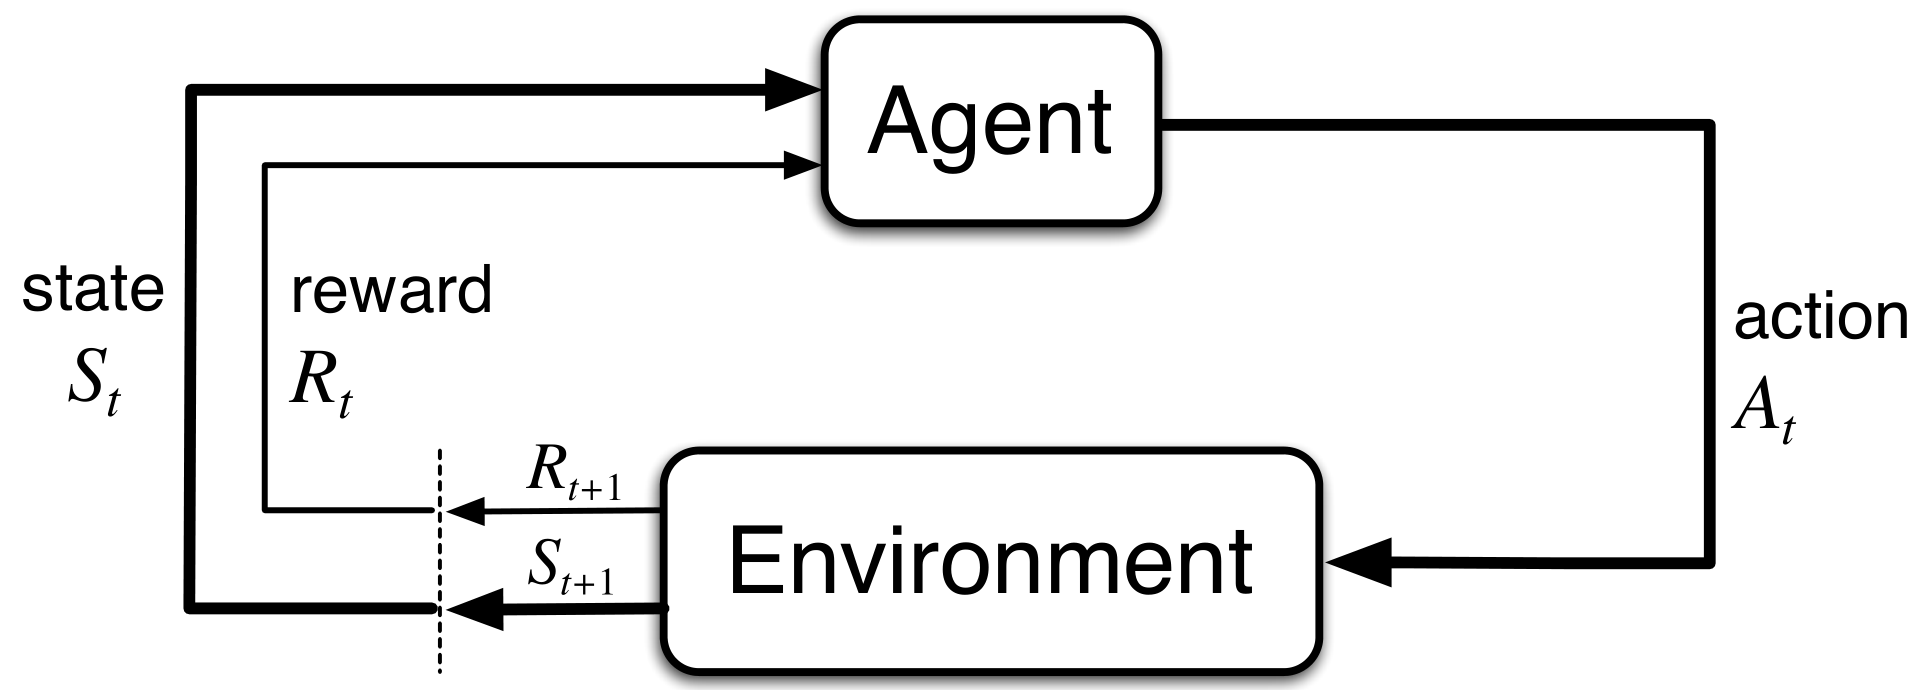
\includegraphics[width=.9\linewidth]{./fig/mdp_interaction.png}
\caption[Markov Decision Process]{The agent-environment interaction in a Markov decision process \cite{sutton18_reinf}}
\end{figure}
\begin{itemize}
\item Classical formulation of sequential decision making
\item Actions influence immediate rewards, but also future rewards
\item Trade-off between immediate and delayed reward
\end{itemize}
\subsubsection{Tabular Methods}
\label{sec:orge9ae482}
\paragraph{Dynamic Programming}
\label{sec:org92189db}
\paragraph{Monte-Carlo Methods}
\label{sec:orga410571}
\paragraph{Temporal-Difference Learning}
\label{sec:org5c9468b}
\begin{enumerate}
\item TD Prediction
\label{sec:org5abb7f1}
\item SARSA: On-policy TD Control
\label{sec:org969082d}
\item Q-learning: Off-policy TD Control
\label{sec:org5770b43}
\end{enumerate}
\paragraph{Q-Learning}
\label{sec:org80c5094}
\subsubsection{Function Approximation}
\label{sec:orge30b02d}
\subsubsection{Exploitation-Exploration Trade-off}
\label{sec:orgeda100e}
\paragraph{\(\epsilon\)-greedy Method}
\label{sec:org24dc8d2}
\subsubsection{Deep Reinforcement Learning}
\label{sec:org87bf818}
\section{Empirical Setting / Data (10\%)}
\label{sec:orgbcc5603}
\subsection{Carsharing Fleets of Electric Vehicles}
\label{sec:org0cb9189}
\subsubsection{Raw Data}
\label{sec:orgcf26099}
The dataset consists of 500 EVs in Stuttgart. As displayed in Table
\ref{car2go-sample-data}, the data contain spatio-temporal attributes, such as
timestamp, coordinates, and address of the EVs. Additionally, status attributes
of the interior and exterior are given, the relative state of charge and
information whether the EV is plugged into one of the 200 charging stations in
Stuttgart.

\begin{longtable}{l|ccccc}
\caption{Raw Car2Go Trip Data from Stuttgart \label{car2go-sample-data}}
\\
\hline
\hline
Number Plate & Latitude & Longitude & Street & Zip Code & Engine Type\\
\hline
\endfirsthead
\multicolumn{6}{l}{Continued from previous page} \\
\hline

Number Plate & Latitude & Longitude & Street & Zip Code & Engine Type \\

\hline
\endhead
\hline\multicolumn{6}{r}{Continued on next page} \\
\endfoot
\endlastfoot
\hline
S-GO2471 & 9.19121 & 48.68895 & Parkplatz Flughafen & 70692 & electric\\
S-GO2471 & 9.15922 & 48.78848 & Salzmannweg 3 & 70192 & electric\\
S-GO2471 & 9.17496 & 48.74928 & Felix-Dahn-Str.45 & 70597 & electric\\
S-GO2471 & 9.17496 & 48.74928 & Felix-Dahn-Str.45 & 70597 & electric\\
S-GO2471 & 9.17496 & 48.74928 & Felix-Dahn-Str.45 & 70597 & electric\\
\hline
Number Plate & Interior & Exterior & Timestamp & Charging & State of Charge\\
\hline
S-GO2471 & good & good & 22.12.2017 20:10 & no & 94\\
S-GO2471 & good & good & 24.12.2017 23:05 & no & 72\\
S-GO2471 & good & good & 26.12.2017 00:40 & yes & 81\\
S-GO2471 & good & good & 26.12.2017 00:45 & yes & 83\\
S-GO2471 & good & good & 26.12.2017 00:50 & yes & 84\\
\hline
\hline
\end{longtable}
\subsubsection{Preprocessing Steps}
\label{sec:org39049ba}
\subsection{Electricity Markets Data}
\label{sec:org37bef3c}
\subsubsection{Secondary Operating Reserve Market}
\label{sec:orgcbde2c2}
\subsubsection{Intraday Continuous Spot Market}
\label{sec:org0dd9e25}

\section{Model: FleetRL (20\%)}
\label{sec:org9ca3858}
\subsection{Information Assumptions}
\label{sec:org7c1da74}
\subsection{Mobility Demand \& Clearing Price Prediction}
\label{sec:org5c95c6d}
\subsection{Reinforcement Learning Approach}
\label{sec:org75dcd95}
\subsection{Bidding Strategy}
\label{sec:org95eefef}
\subsection{Dispatch Heuristic / Algorithm}
\label{sec:orgf5e70dc}

\section{Evaluation (30\%)}
\label{sec:orgadc21db}
\subsection{Event-based Simulation}
\label{sec:org2d89c25}
\subsection{Benchmark: Ad-hoc Strategies}
\label{sec:orge6ab547}
\subsection{FleetRL}
\label{sec:org636337b}
\subsection{Sensitivity Analysis: Prediction Accuracy}
\label{sec:org4a56efa}
\subsection{Sensitivity Analysis: Infrastructure Changes}
\label{sec:orgb67fd8a}
\subsection{Sensitivity Analysis: Bidding Strategy}
\label{sec:orgb3ee576}
\section{Discussion (5\%)}
\label{sec:org68e059a}
\subsection{Generalizability}
\label{sec:org962e037}
\subsection{Future Electricity Landscape}
\label{sec:orgf0ba672}
\subsection{Limitations}
\label{sec:org7cfb617}
\section{Conclusion (5\%)}
\label{sec:org7f769c5}
\subsection{Contribution}
\label{sec:orgf3396c4}
\subsection{Future Research}
\label{sec:org3574a59}


\bibliography{bibliography/references}
\bibliographystyle{apacite}
\end{document}
